\subsection{Appearance attributes extraction}
\label{sec:vehcol_extraction}
We build two modules, color encoder $E_{col}$ and vehicle encoder $E_{veh}$, with EfficientNet \cite{tan2019efficientnet} backbone to learn the visual features representation for each target vehicle from the video tracks.
The encoders are trained as a classification task, which takes the target bounding boxes as input and learns to classify them to the most reasonable groups extracted from the previous query processing step (section \ref{sec:text_extraction}). \\
\begin{figure}[!h]
    \centering
    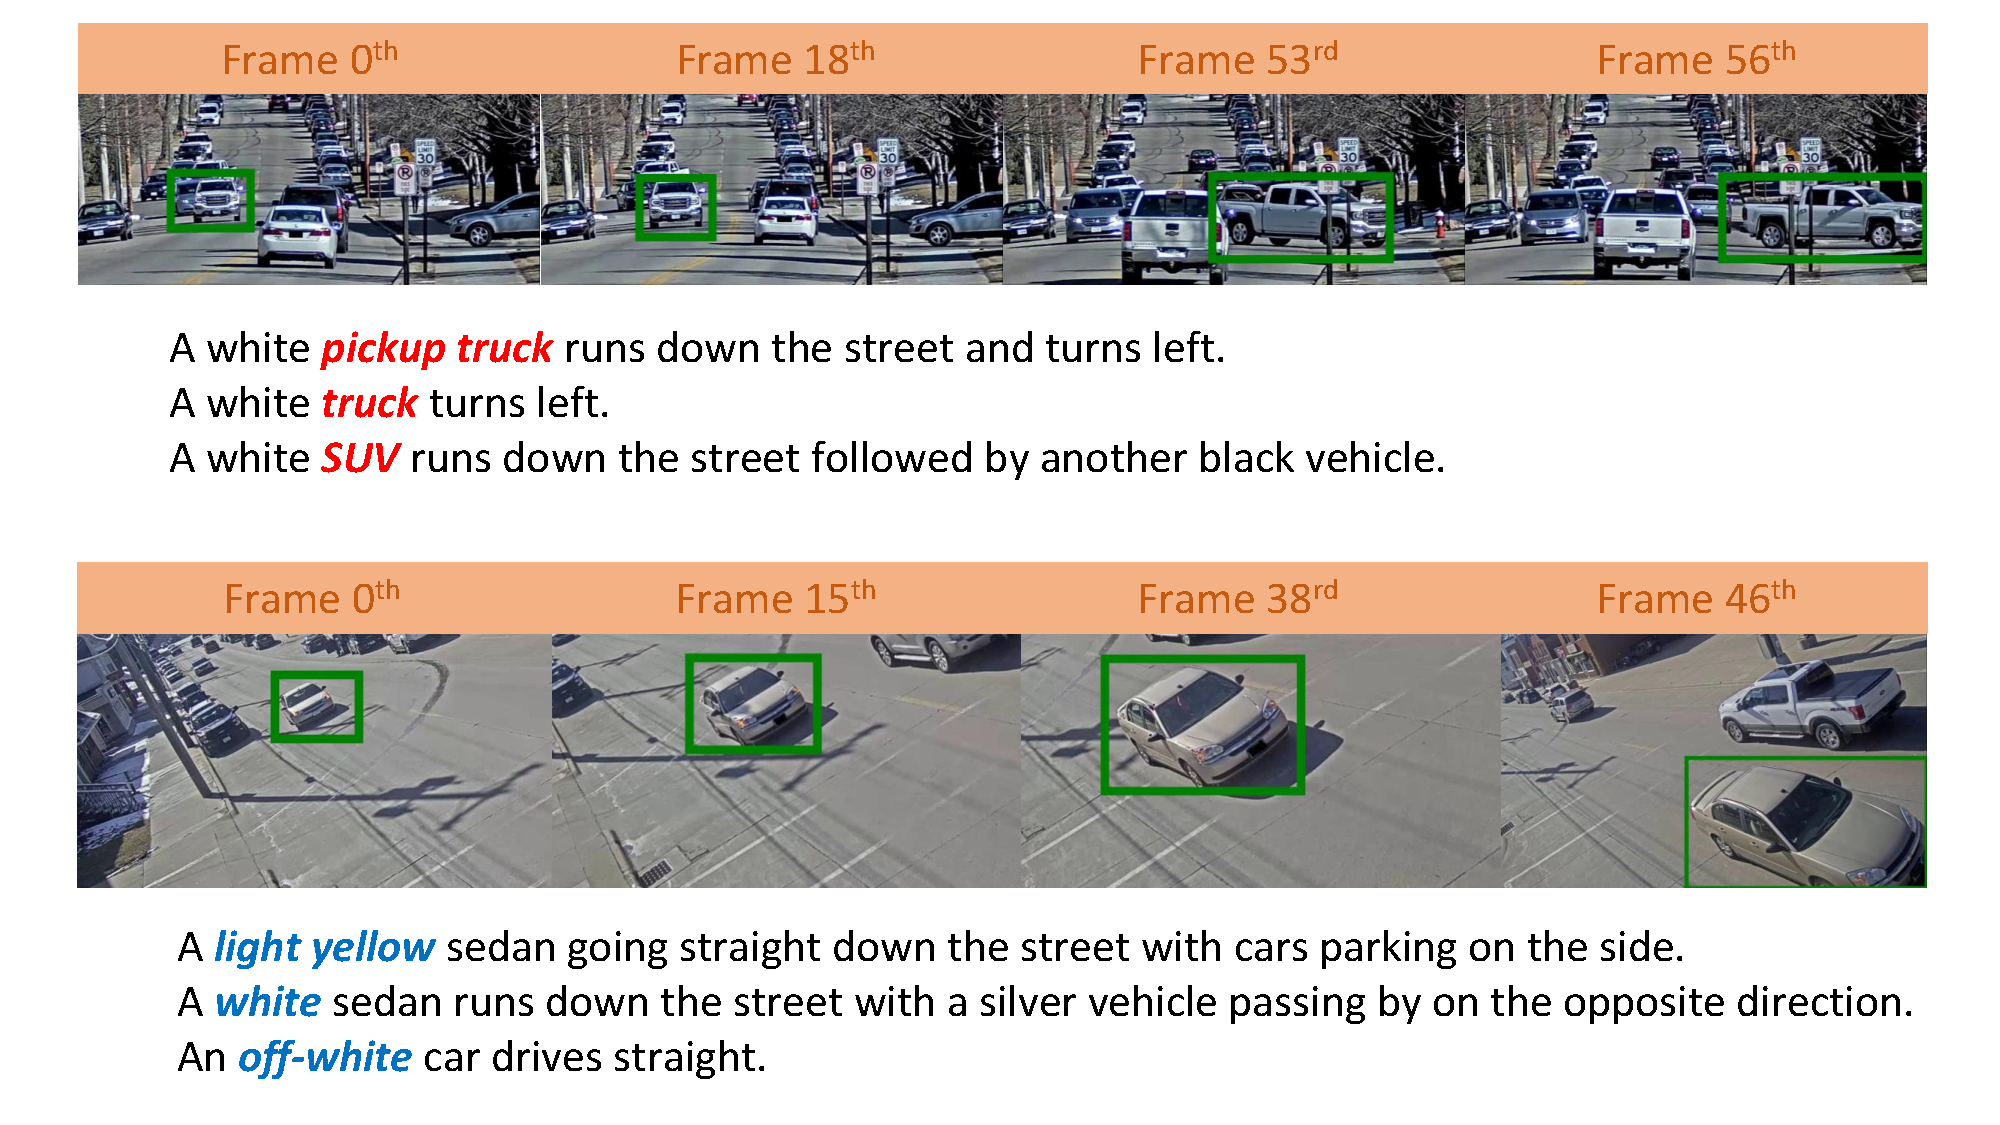
\includegraphics[width=\textwidth]{resources/images/methods/hard_classification.pdf}
    \caption{Examples of ambiguous color/vehicle type labelling affected by different viewpoints or external influences.}
    \label{fig:hard_color}
\end{figure}
\begin{figure}[!h]
    \centering
    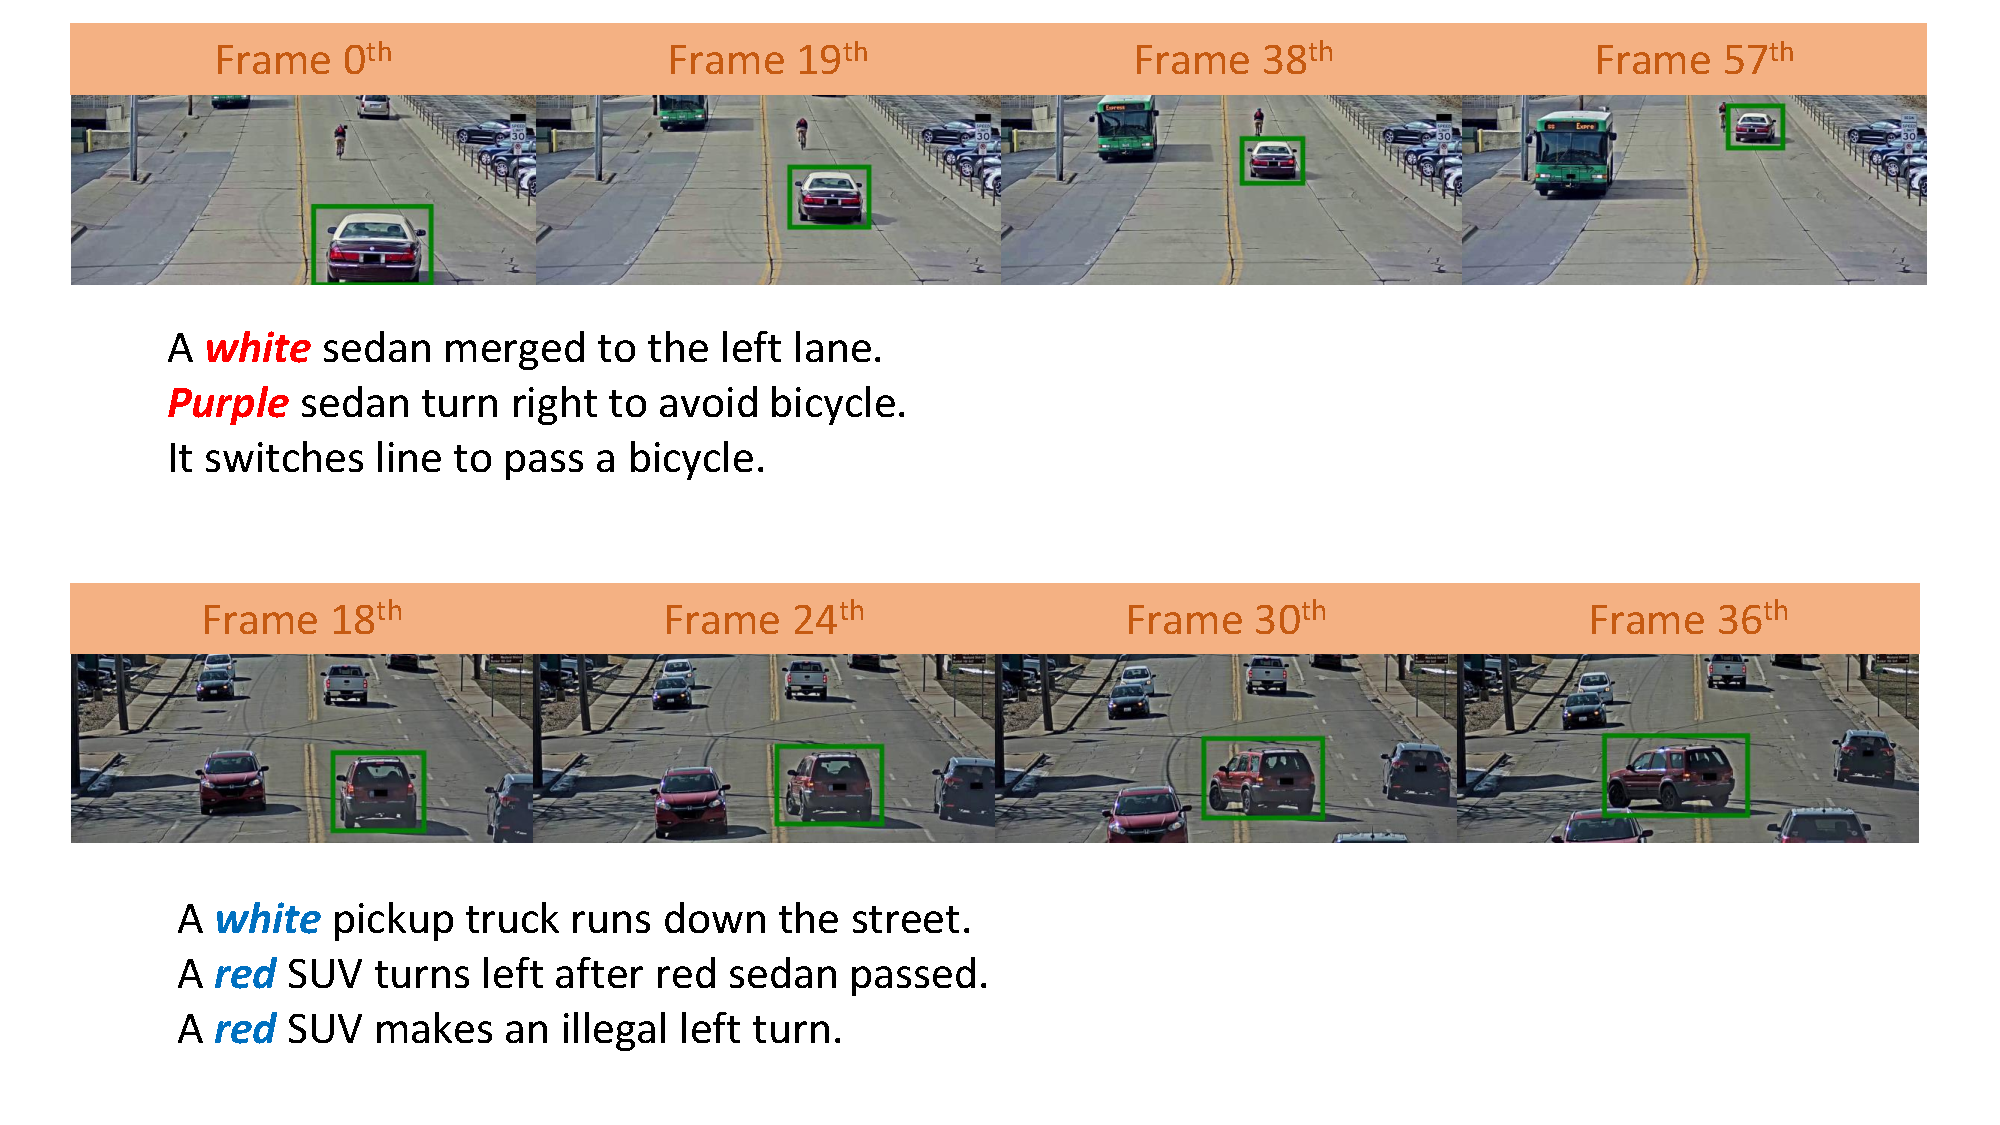
\includegraphics[width=\textwidth]{resources/images/methods/multicolor_example.pdf}
    \caption{Examples of multi-color vehicles.}
    \label{fig:multicolor}
\end{figure}
However, in practice, the vehicle's visual attributes are not consistent between different viewpoints or could be easily affected by external conditions (sunlight, dust), as pointed in Figure \ref{fig:hard_color}. 
Also, there are some cases the vehicle itself has multi-color, as shown in Figure \ref{fig:multicolor}.
Therefore, instead of labeling each main subject with a specific class, we gather all textual attributes provided by the three captions as the multi-label ground-truth for each target. Then, we train the classifiers with multi-label approaches, where a sigmoid function replaces the softmax activation in the classification layer. \\
About the training images, for a given track with $T$ frames and $T$ temporal bounding boxes, we sample four boxes: $[B_0, B_{T/3}, B_{2T/3}, B_{T-1}]$ to handle this problem.